% ============================================================================
% AD7031 Homework 1 -- Solutions.  Same preamble as hw01.tex plus tikz/listings,
% kotex for the plain-Korean answers in Problem 4, and a blue `solution'
% environment.  Self-contained; compiles with pdflatex.
% All numbers were checked with independent gurobipy runs (Gurobi 12).
% ============================================================================
\documentclass[10pt]{article}

\usepackage[a4paper, margin=2.2cm]{geometry}
\usepackage{amsmath, amssymb}
\usepackage[dvipsnames]{xcolor}
\usepackage{array}
\usepackage{enumitem}
\usepackage{tikz}
\usepackage{listings}
\usepackage{needspace}
\usepackage{kotex}
\usepackage[hidelinks]{hyperref}

\definecolor{ruleink}{RGB}{18, 68, 140}
\definecolor{solink}{RGB}{20, 60, 170}

\setlength{\parindent}{0pt}
\pagestyle{plain}

\AtBeginDocument{%
  \abovedisplayskip=5pt plus 1pt
  \belowdisplayskip=5pt plus 1pt
  \abovedisplayshortskip=3pt
  \belowdisplayshortskip=3pt}

\lstset{basicstyle=\ttfamily\small, columns=fullflexible, keepspaces=true,
  xleftmargin=1em, aboveskip=4pt, belowskip=4pt}

% ---- one problem -----------------------------------------------------------
\newcommand{\problem}[2]{%   points, title
  \par\bigskip
  {\color{ruleink}\rule{\textwidth}{1pt}}\par\nobreak\vspace{3pt}
  {\large\bfseries #2}\hfill{\normalsize\bfseries(#1 points)}\par\nobreak\vspace{4pt}}

\newlist{parts}{enumerate}{1}
\setlist[parts]{label=(\alph*), leftmargin=2.2em, itemsep=3pt}

% ---- solution block ----------------------------------------------------------
\newenvironment{solution}
  {\par\smallskip\begingroup\color{solink}\textbf{Solution.}\ }
  {\endgroup\par}

\begin{document}

\begin{center}
  {\large AD7031 Optimization Under Uncertainty}\\[3pt]
  {\Large\bfseries Homework 1 --- Solutions}\\[4pt]
  {\small \textbf{Due Sep 26, start of class}}
\end{center}
\medskip\hrule\medskip

% ================================================================ Problem 1
\problem{40}{Problem 1. From words to a model}

A transport aircraft is being loaded for a resupply flight. Two cargo types, with value,
weight and volume given per pallet:

\begin{center}
\begin{tabular}{l|cc}
              & ammunition & fuel \\ \hline
 value (pts)  & 4 & 5 \\
 weight (t)   & 3 & 2 \\
 volume (m$^3$) & 1 & 3 \\
\end{tabular}
\end{center}

The aircraft carries at most $60$ t and $48$ m$^3$, and orders require that at least
$3$ pallets of ammunition fly. Cargo is divisible --- fractional pallets are allowed.
The goal is to maximize total value.

\begin{parts}
\item \textbf{(8 pts)} Define the decision variables and write the problem as a scalar
  LP --- objective and constraints, one line each, with a few words saying what each
  constraint enforces.

\begin{solution}
Let $x_a$ be the number of ammunition pallets loaded and $x_f$ the number of fuel
pallets, both real numbers.
\[
\begin{aligned}
  \max\quad & 4x_a + 5x_f && \text{total value} \\
  \text{s.t.}\quad & 3x_a + 2x_f \le 60 && \text{weight limit (t)} \\
                   & x_a + 3x_f \le 48 && \text{volume limit (m$^3$)} \\
                   & x_a \ge 3 && \text{minimum ammunition order} \\
                   & x_a, x_f \ge 0 && \text{no negative cargo}
\end{aligned}
\]
\end{solution}

\item \textbf{(8 pts)} Now put that LP in the Week 2 canonical vector form
  $\max\, c^{\top}x$ s.t.\ $Ax \le b$: write out $c$, $A$, $b$ with numbers in them, and
  report the dimensions of $A$.

\begin{solution}
Take $x = (x_a, x_f)^{\top}$. The order $x_a \ge 3$ becomes $-x_a \le -3$, and
$x_f \ge 0$ becomes $-x_f \le 0$. The row $x_a \ge 0$ is implied by $x_a \ge 3$, so it
can be dropped:
\[
c = \begin{pmatrix} 4 \\ 5 \end{pmatrix}, \qquad
A = \begin{pmatrix}
  3 & 2 \\
  1 & 3 \\
  -1 & 0 \\
  0 & -1
\end{pmatrix}, \qquad
b = \begin{pmatrix} 60 \\ 48 \\ -3 \\ 0 \end{pmatrix}
\qquad
\begin{array}{l}
  \scriptstyle\text{weight} \\ \scriptstyle\text{volume} \\
  \scriptstyle x_a \ge 3 \\ \scriptstyle x_f \ge 0
\end{array}
\]
$A$ is $4 \times 2$: four constraints, two variables. Keeping the redundant row
$-x_a \le 0$ as well gives a $5 \times 2$ matrix that describes the same feasible set;
either answer is fine, as long as the dimension reported matches the matrix written.
\end{solution}

\item \textbf{(14 pts)} Solve it by picture. Draw the feasible region in Desmos and
  include a screenshot. Then list every vertex with its coordinates and its objective
  value, and report the optimal solution and its optimal value.

\begin{solution}
In Desmos, type the four inequalities as they stand, with $x = x_a$ and $y = x_f$:
\texttt{3x+2y<=60}, \texttt{x+3y<=48}, \texttt{x>=3}, \texttt{y>=0}. The region where
all four shadings overlap is the feasible set --- the quadrilateral below.
\par\medskip
\begin{center}
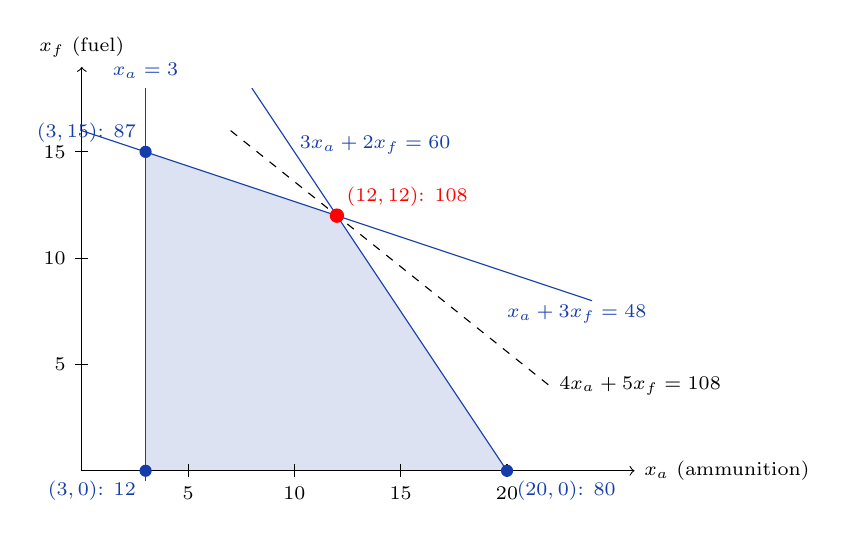
\begin{tikzpicture}[x=0.27cm, y=0.27cm, every node/.style={font=\scriptsize}]
  \fill[solink!15] (3,0) -- (20,0) -- (12,12) -- (3,15) -- cycle;
  \draw[->] (0,0) -- (26,0) node[right] {$x_a$ (ammunition)};
  \draw[->] (0,0) -- (0,19) node[above] {$x_f$ (fuel)};
  \foreach \i in {5,10,15,20} { \draw (\i,0.3) -- (\i,-0.3) node[below] {\i}; }
  \foreach \i in {5,10,15} { \draw (0.3,\i) -- (-0.3,\i) node[left] {\i}; }
  \draw[solink] (20,0) -- (8,18) node[pos=0.85, right] {$3x_a + 2x_f = 60$};
  \draw[solink] (0,16) -- (24,8) node[pos=0.97, below] {$x_a + 3x_f = 48$};
  \draw[solink] (3,-0.5) -- (3,18) node[above] {$x_a = 3$};
  \draw[dashed] (7,16) -- (22,4) node[pos=1, right] {$4x_a + 5x_f = 108$};
  \fill[solink] (3,0) circle (2.2pt) node[below left] {$(3,0)$: 12};
  \fill[solink] (20,0) circle (2.2pt) node[below right] {$(20,0)$: 80};
  \fill[solink] (3,15) circle (2.2pt) node[above left] {$(3,15)$: 87};
  \fill[red] (12,12) circle (2.6pt) node[above right, text=red] {$(12,12)$: 108};
\end{tikzpicture}
\end{center}
The four vertices, each with $4x_a + 5x_f$:
\begin{center}
\begin{tabular}{l|l|c}
 vertex & which two constraints meet there & value \\ \hline
 $(3,0)$   & $x_a = 3$ and $x_f = 0$              & $12$ \\
 $(20,0)$  & weight and $x_f = 0$                 & $80$ \\
 $(12,12)$ & weight and volume                    & $\mathbf{108}$ \\
 $(3,15)$  & volume and $x_a = 3$                 & $87$ \\
\end{tabular}
\end{center}
The optimum is $x_a^{\star} = 12$, $x_f^{\star} = 12$ with value $108$. The dashed
line is the objective level set through the optimum: pushing it any further up and to
the right leaves the region, which is why the optimum sits at that corner.
\end{solution}

\item \textbf{(10 pts)} Implement the LP with \texttt{gurobipy} and solve it. Include a
  screenshot of your code and its printed output. Check that Gurobi agrees with (c).

\Needspace{16\baselineskip}
\begin{solution}
\begin{lstlisting}
import gurobipy as gp
from gurobipy import GRB

model = gp.Model("cargo")
x_ammo = model.addVar(vtype=GRB.CONTINUOUS, name="x_ammo")   # lower bound 0 by default
x_fuel = model.addVar(vtype=GRB.CONTINUOUS, name="x_fuel")
model.setObjective(4 * x_ammo + 5 * x_fuel, GRB.MAXIMIZE)
model.addConstr(3 * x_ammo + 2 * x_fuel <= 60, name="weight")
model.addConstr(x_ammo + 3 * x_fuel <= 48, name="volume")
model.addConstr(x_ammo >= 3, name="min_ammo")
model.optimize()

print(f"optimal solution ammunition is {x_ammo.X}")
print(f"optimal solution fuel is {x_fuel.X}")
print(f"optimal objective value is {model.ObjVal}")
\end{lstlisting}
Output:
\begin{lstlisting}
optimal solution ammunition is 12.0
optimal solution fuel is 12.0
optimal objective value is 108.0
\end{lstlisting}
Gurobi returns $(12, 12)$ with value $108$, the same corner as the drawing in (c).
\end{solution}
\end{parts}

% ================================================================ Problem 2
\problem{20}{Problem 2. Convex sets}

\begin{parts}
\item \textbf{(10 pts)} Draw two convex sets in $\mathbb{R}^2$ whose \emph{union} is not
  convex, marking two points and the point on their segment that escapes. Then
  \emph{try} to draw two convex sets whose \emph{intersection} is not convex.

\Needspace{14\baselineskip}
\begin{solution}
\par\medskip
\begin{center}
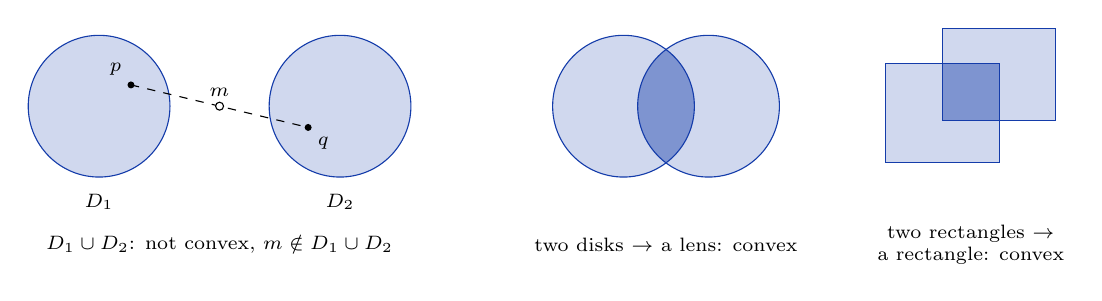
\begin{tikzpicture}[scale=0.9, every node/.style={font=\scriptsize}]
  % union: two disks that do not touch
  \fill[solink!20] (0,0) circle (1.0);
  \fill[solink!20] (3.4,0) circle (1.0);
  \draw[solink] (0,0) circle (1.0);
  \draw[solink] (3.4,0) circle (1.0);
  \node at (0,-1.35) {$D_1$};
  \node at (3.4,-1.35) {$D_2$};
  \fill (0.45,0.3) circle (1.4pt) node[above left] {$p$};
  \fill (2.95,-0.3) circle (1.4pt) node[below right] {$q$};
  \draw[dashed] (0.45,0.3) -- (2.95,-0.3);
  \draw[fill=white] (1.7,0) circle (1.6pt) node[above] {$m$};
  \node at (1.7,-1.95) {$D_1 \cup D_2$: not convex, $m \notin D_1 \cup D_2$};
  % intersection attempts: lens, and rectangle
  \begin{scope}[xshift=7.4cm]
    \fill[solink!20] (0,0) circle (1.0);
    \fill[solink!20] (1.2,0) circle (1.0);
    \begin{scope}
      \clip (0,0) circle (1.0);
      \fill[solink!55] (1.2,0) circle (1.0);
    \end{scope}
    \draw[solink] (0,0) circle (1.0);
    \draw[solink] (1.2,0) circle (1.0);
    \node at (0.6,-1.95) {two disks $\to$ a lens: convex};
  \end{scope}
  \begin{scope}[xshift=12.2cm]
    \fill[solink!20] (-1.1,-0.8) rectangle (0.5,0.6);
    \fill[solink!20] (-0.3,-0.2) rectangle (1.3,1.1);
    \fill[solink!55] (-0.3,-0.2) rectangle (0.5,0.6);
    \draw[solink] (-1.1,-0.8) rectangle (0.5,0.6);
    \draw[solink] (-0.3,-0.2) rectangle (1.3,1.1);
    \node[align=center] at (0.1,-1.95) {two rectangles $\to$\\ a rectangle: convex};
  \end{scope}
\end{tikzpicture}
\end{center}
Left: $D_1$ and $D_2$ are convex, but $p \in D_1$, $q \in D_2$, and the midpoint $m$ of
their segment lies in the gap between them, so the union fails the segment test.
Right: every attempt at a non-convex intersection fails --- two disks meet in a lens,
two rectangles in a rectangle, both convex. This is not bad luck: the intersection of
convex sets is always convex (a segment that stays inside each set stays inside their
common part).
\end{solution}

\item \textbf{(10 pts)} Show that a polyhedron $P = \{\, x \in \mathbb{R}^n : Ax \le b \,\}$
  is a convex set.

\begin{solution}
Take $x, y \in P$, so $Ax \le b$ and $Ay \le b$, and $\lambda \in [0,1]$. Then
\[
  A\big(\lambda x + (1-\lambda) y\big)
  = \lambda\, Ax + (1-\lambda)\, Ay
  \;\le\; \lambda\, b + (1-\lambda)\, b
  = b ,
\]
where the inequality holds row by row because $\lambda \ge 0$ and $1 - \lambda \ge 0$:
multiplying an inequality by a nonnegative number keeps its direction, and adding two
inequalities of the same direction is allowed. So $\lambda x + (1-\lambda) y \in P$, and
$P$ passes the segment test.
\end{solution}
\end{parts}

% ================================================================ Problem 3
\problem{20}{Problem 3. Convex functions}

\begin{parts}
\item \textbf{(10 pts)} Suppose $f_k : \mathbb{R}^N \to \mathbb{R}$, $k \in [K]$, are
  convex. Show that $g(x) = \sum_{k} f_k(x)$ and $g(x) = \max_{k} f_k(x)$ are convex.

\begin{solution}
Fix $x, y \in \mathbb{R}^N$ and $\lambda \in [0,1]$, and write $z = \lambda x + (1-\lambda) y$.
\par\smallskip
\emph{Sum.} Apply the definition to each $f_k$ and add the $K$ inequalities:
\[
  g(z) = \sum_{k} f_k(z)
  \;\le\; \sum_{k} \big[\lambda f_k(x) + (1-\lambda) f_k(y)\big]
  = \lambda \sum_{k} f_k(x) + (1-\lambda) \sum_{k} f_k(y)
  = \lambda g(x) + (1-\lambda) g(y).
\]
\emph{Max.} For every single $k$,
\[
  f_k(z) \;\le\; \lambda f_k(x) + (1-\lambda) f_k(y)
  \;\le\; \lambda \max_{j} f_j(x) + (1-\lambda) \max_{j} f_j(y)
  = \lambda g(x) + (1-\lambda) g(y),
\]
because replacing $f_k(x)$ by the largest of the $f_j(x)$ can only increase the right-hand
side. The right-hand side does not depend on $k$, so taking the max over $k$ on the left
gives $g(z) \le \lambda g(x) + (1-\lambda) g(y)$.
\end{solution}

\item \textbf{(5 pts)} Show that $f(x) = x^2$ is convex.

\begin{solution}
For $x, y \in \mathbb{R}$ and $\lambda \in [0,1]$, expand the difference between the two
sides of the definition:
\[
  \lambda x^2 + (1-\lambda) y^2 - \big(\lambda x + (1-\lambda) y\big)^2
  = \lambda(1-\lambda)\,x^2 - 2\lambda(1-\lambda)\,xy + \lambda(1-\lambda)\,y^2
  = \lambda(1-\lambda)\,(x-y)^2 \;\ge\; 0 ,
\]
since $\lambda \ge 0$, $1-\lambda \ge 0$ and a square is nonnegative. Hence
$(\lambda x + (1-\lambda) y)^2 \le \lambda x^2 + (1-\lambda) y^2$. (Writing ``$=$''
here is the common slip: the two sides are equal only when $x = y$.)
\end{solution}

\item \textbf{(5 pts)} Show that $f(x) = \|x\|_2^2$ is convex.

\begin{solution}
$\|x\|_2^2 = x_1^2 + x_2^2 + \cdots + x_N^2$ is a sum of the $N$ functions
$f_i(x) = x_i^2$. Each $f_i$ is convex by (b) applied to the $i$-th coordinates:
$(\lambda x_i + (1-\lambda) y_i)^2 \le \lambda x_i^2 + (1-\lambda) y_i^2$. A sum of
convex functions is convex by (a). So $\|x\|_2^2$ is convex.
\end{solution}
\end{parts}

% ================================================================ Problem 4
\problem{20}{Problem 4. Markowitz portfolio}

Three funds --- bond, tech, energy --- with mean vector $\mu$ and covariance matrix
$\Sigma$:
\[
  \mu = \begin{pmatrix} 0.06 \\ 0.10 \\ 0.15 \end{pmatrix},
  \qquad
  \Sigma = \begin{pmatrix}
    0.010 & 0.001 & 0.000 \\
    0.001 & 0.040 & 0.015 \\
    0.000 & 0.015 & 0.090
  \end{pmatrix},
  \qquad
  \begin{aligned}
    \min_{x \in \mathbb{R}^3} \quad & x^{\top}\Sigma x \\
    \text{s.t.} \quad & \mu^{\top}x \ge r, \quad \mathbf{1}^{\top}x = 1, \quad x \ge 0 .
  \end{aligned}
\]

\begin{parts}
\item \textbf{(15 pts)} Choose your own minimum mean return $r$, implement the model with
  \texttt{gurobipy}, and print the result. Is your problem feasible? If it is, raise $r$
  until it stops being feasible, report that $r$, and explain why --- in plain Korean.

\Needspace{18\baselineskip}
\begin{solution}
With $r = 0.10$ (any choice is fine; what matters is the reasoning that follows):
\begin{lstlisting}
import gurobipy as gp
from gurobipy import GRB

model = gp.Model("markowitz")
x_bond   = model.addVar(vtype=GRB.CONTINUOUS, name="x_bond")
x_tech   = model.addVar(vtype=GRB.CONTINUOUS, name="x_tech")
x_energy = model.addVar(vtype=GRB.CONTINUOUS, name="x_energy")

# objective -- portfolio variance x' Sigma x, written out term by term
model.setObjective(
    0.010 * x_bond * x_bond
    + 0.040 * x_tech * x_tech
    + 0.090 * x_energy * x_energy
    + 2 * 0.001 * x_bond * x_tech
    + 2 * 0.015 * x_tech * x_energy,
    GRB.MINIMIZE,
)
r = 0.10
model.addConstr(0.06 * x_bond + 0.10 * x_tech + 0.15 * x_energy >= r, name="target_return")
model.addConstr(x_bond + x_tech + x_energy == 1, name="budget")   # the whole fund is invested
model.optimize()

print(f"optimal solution bond is {x_bond.X}")
print(f"optimal solution tech is {x_tech.X}")
print(f"optimal solution energy is {x_energy.X}")
print(f"optimal objective value is {model.ObjVal}")
\end{lstlisting}
Output:
\begin{lstlisting}
optimal solution bond is 0.3922872131614318
optimal solution tech is 0.2938830159484385
optimal solution energy is 0.31382977089013236
optimal objective value is 0.016855053202895175
\end{lstlisting}
So $r = 0.10$ is \textbf{feasible}: about $39\%$ bond, $29\%$ tech, $31\%$ energy, with
variance $0.0169$ (standard deviation $\approx 0.13$). Note the budget row is
\texttt{==\,1}, as the model states; the Week 3 notebook's \texttt{<=\,1} is a different
model (the leftover sits in cash) and gives a different portfolio for the same $r$.
\par\smallskip
Raising $r$ and re-solving:
\begin{center}
\begin{tabular}{c|ccc|c|l}
 $r$ & bond & tech & energy & variance & \\ \hline
 $0.10$  & $0.392$ & $0.294$ & $0.314$ & $0.0169$ & feasible \\
 $0.12$  & $0.116$ & $0.392$ & $0.493$ & $0.0340$ & feasible \\
 $0.14$  & $0$     & $0.200$ & $0.800$ & $0.0640$ & feasible \\
 $0.15$  & $0$     & $0$     & $1$     & $0.0900$ & feasible --- everything in energy \\
 $0.151$ & \multicolumn{3}{c|}{---} & --- & \textbf{infeasible} (Gurobi: \texttt{Model is infeasible}) \\
\end{tabular}
\end{center}
The problem stops being feasible as soon as $r$ exceeds $0.15$: $r = 0.15$ is the last
feasible value, and $r = 0.151$ (or any $r > 0.15$) has no solution.
\par\smallskip
\emph{Why, in plain Korean.}
돈을 세 펀드에 어떻게 나누어 넣더라도, 포트폴리오 전체의 기대수익률은 세 펀드 중 기대수익률이
가장 높은 에너지 펀드의 15\%를 넘을 수 없습니다. 가장 좋은 펀드 하나에 전부 넣는 것이 기대수익률을
가장 높이는 방법이고, 그때가 딱 15\%이기 때문입니다. 그래서 요구 수익률 $r$이 15\%를 넘는 순간, 어떤
배분도 조건을 만족하지 못해 문제가 풀리지 않습니다 (infeasible). 반대로 $r$이 작을수록 (예: $0.01$)
조건은 느슨해지고, 답은 변동성이 가장 작은 배분으로 갑니다.
\end{solution}

\item \textbf{(5 pts)} Is the Markowitz problem a convex problem? If it is, explain why.

\begin{solution}
Yes. \emph{Objective.} $f(x) = x^{\top}\Sigma x$ is convex because $\Sigma$ is a
covariance matrix, hence positive semidefinite ($v^{\top}\Sigma v \ge 0$ for every $v$
--- it is the variance of the portfolio $v$). Repeating the computation of Problem 3(b)
with vectors,
\[
  \lambda f(x) + (1-\lambda) f(y) - f\big(\lambda x + (1-\lambda) y\big)
  = \lambda(1-\lambda)\,(x-y)^{\top}\Sigma\,(x-y) \;\ge\; 0 .
\]
\emph{Feasible set.} $\{\, x : \mu^{\top}x \ge r,\ \mathbf{1}^{\top}x = 1,\ x \ge 0 \,\}$ is
described by linear inequalities and one linear equality ($= 1$ is $\le 1$ and $\ge 1$
together), so it is a polyhedron, which is convex by Problem 2(b). A convex objective over
a convex feasible set is a convex problem --- which is why Gurobi finds the global optimum
without any search.
\end{solution}
\end{parts}

\end{document}
